\section{Упорядоченные деревья (деревья поиска). Поиск в упорядоченном дереве.  Сбалансированное дерево}
\section{Методы балансировки (самобаоансировки) деревьев}
\section{Поиск в линейных коллекциях (массивах, списках): линейный, дихотомический, поиск скачками, интерполяционный}
\section{Поиск в многомерных массивах}
\section{Нечеткий поиск - поиск подобной подстроки}
Задача нечеткого поиска (fuzzy string search)~--- найти в тексте или словаре (\textit{haystack}) все подстроки, совпадающие
(начинающиеся) с данной (\textit{needle}) с учетом не более \(k\) ошибок.
Эти алгоритмы являются основными в системах коррекции наборных ошибок
(например \href{https://en.wikipedia.org/wiki/Code_completion}{автодополнение кода} в IDE или подсказки в поисковой строке браузера).
В зависимости от преследуемых целей, существуют и используются различные алгоритмы решения данной задачи в различных постановках.

\subsubsection{Метрики Левенштейна и Хэмминга}
Расстояние Левенштейна~--- минимальное количество односимвольных операций (а именно вставки, удаления, замены),
необходимых для превращения одной последовательности символов в другую.
% cSpell: disable-next-line
Например, расстояние Левенштейна слов \(L(Hello, Hilo) = 2\) (замена `\(e\)' \(\gets\) `\(i\)', вставка `\(l\)').

Расстояние Хэмминга~--- число позиций, в которых соответствующие символы двух слов одинаковой длины различны. Например,
% cSpell: disable-next-line
\(H(Hello, Hillo) = 1\) (замена `\(e\)' \(\gets\) `\(i\)').

Расстояния Хэмминга и Левенштейна, во-первых, являются метриками в математическом смысле слова, во-вторых, позволяют строго
формализовать задачу нечеткого поиска.

Расстояние Левенштейна можно вычислить на основе рекуррентной формулы \[L(a,b) = \begin{cases}
    |a|                                  & \text{если}~|b| = 0,                         \\
    |b|                                  & \text{если}~|a| = 0,                         \\
    L(\text{tail}(a), \text{tail}(b))    & \text{если}~\text{head}(a) = \text{head}(b), \\
    1 + \min \begin{cases}
               L(\text{tail}(a), b)              \\
               L(a, \text{tail}(b))              \\
               L(\text{tail}(a), \text{tail}(b)) \\
             \end{cases} & \text{иначе}                                          \\
  \end{cases}
\]

где \(\text{tail}(\overline{x_1x_2x_3\dots}) = \overline{x_2x_3\dots}\), а \(\text{head}(\overline{x_1x_2x_3\dots}) = x_1\).
Используя также мемоизацию на матрице, можно вычислить расстояние Левенштейна между любыми двумя строками длины \(n\) и \(m\) за
\(O(n\cdot m)\)~--- алгоритм \href{https://neerc.ifmo.ru/wiki/index.php?title=%D0%97%D0%B0%D0%B4%D0%B0%D1%87%D0%B0_%D0%BE_%D1%80%D0%B5%D0%B4%D0%B0%D0%BA%D1%86%D0%B8%D0%BE%D0%BD%D0%BD%D0%BE%D0%BC_%D1%80%D0%B0%D1%81%D1%81%D1%82%D0%BE%D1%8F%D0%BD%D0%B8%D0%B8,_%D0%B0%D0%BB%D0%B3%D0%BE%D1%80%D0%B8%D1%82%D0%BC_%D0%92%D0%B0%D0%B3%D0%BD%D0%B5%D1%80%D0%B0-%D0%A4%D0%B8%D1%88%D0%B5%D1%80%D0%B0}{Вагнера-Фишера}.

\subsubsection{Алгоритм bitap}
Алгоритм \href{https://en.wikipedia.org/wiki/Bitap_algorithm}{bitap} позволяет эффективно с точки зрения реального времени работы процессора вычислять расстояние Хэмминга и
(с модификациями) Левенштейна. При асимптотике \(O(k\cdot n)\), он работает ощутимо быстрее наивного вычисления метрики
Левенштейна для сравнения двух строк, поскольку сравнивает по 32/64 символа за раз. Фактически, это эффективное
распараллеливание наивного линейного алгоритма.

\subsubsection{Алгоритм расширенной выборки}
\begin{center}
  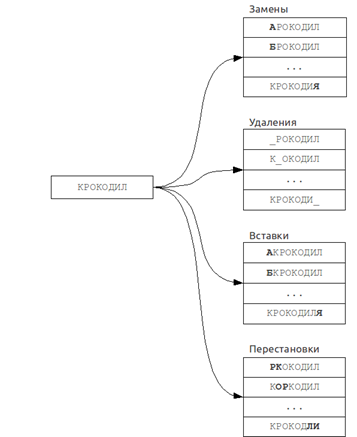
\includegraphics[width=0.3\textwidth]{resources/19-26/inflate.png}
\end{center}
Сводит задачу нечеткого поиска к задаче точного поиска последовательным перебором всех ошибочных трансформаций входной строки.
Неэффективен на больших алфавитах и при больших \(k\), даже при бинарном поиске по словарю временная сложность
\(O((m\cdot |\Sigma|)^k\cdot m\cdot \log{n})\), где \(|\Sigma|\)~--- размер алфавита.

\subsubsection{Метод \(N\)-грамм}
\begin{center}
  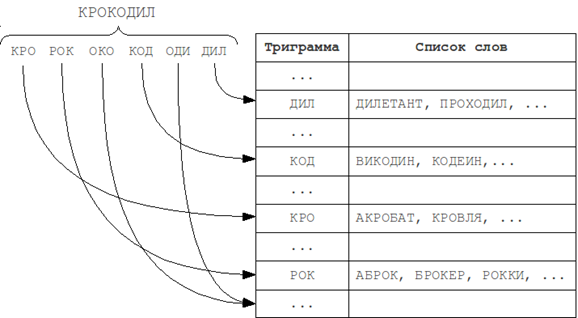
\includegraphics[width=0.3\textwidth]{resources/19-26/n-gramms.png}
\end{center}

Основан на разбиении всех слов в словаре и исходного на \(N\)-граммы~--- последовательности длины \(N\) (обычно \(N = 3\)).
\(N\)-граммы используются для группировки слов в корзины, по которым в дальнейшем и производится поиск.

\subsubsection{\href{https://cs.msu.ru/sites/cmc/files/docs/boycov.pdf}{Хеширование по сигнатуре}, \href{https://en.wikipedia.org/wiki/Locality-sensitive_hashing\#Bit_sampling_for_Hamming_distance}{Locality-sensitive hashing}}

\begin{center}
  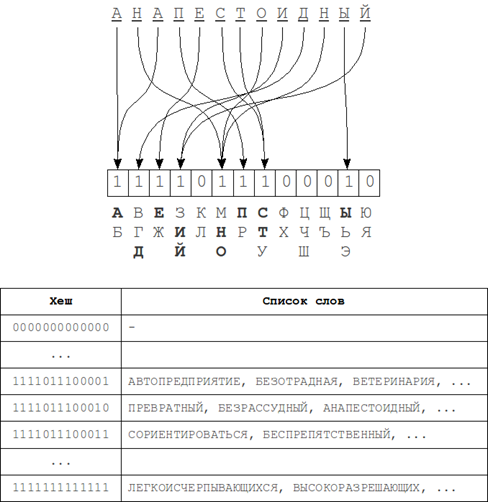
\includegraphics[width=0.3\textwidth]{resources/19-26/hash.png}
\end{center}
Предполагают сопоставление каждому слову специального хеша так, что схожие слова имеют схожие хеш-функции. Тогда поиск следует вести с
теми словами в словаре, у которых близкий или одинаковый хеш с исходной строкой.
\section{Методы сортировки (для линейных коллекций): сортировка вставкой (включением), выбором (выделением), обменом}
\section{Методы сортировки (для линейных коллекций): сортировка слиянием, "быстрая" сортировка Хоара (quicksort)}
